\documentclass[border=8pt]{standalone}
\usepackage{tikz}
\definecolor{bg}{HTML}{171D2B}
\definecolor{acc}{HTML}{F7B538}
\begin{document}
\pagecolor{bg}
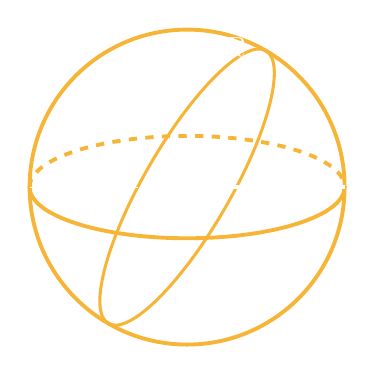
\begin{tikzpicture}[line width=1.4pt, text=white]
  % bola utama
  \draw[acc] (0,0) circle (2);
  % ekuator: depan solid, belakang putus-putus
  \draw[acc] (-2,0) arc[start angle=180, end angle=360, x radius=2, y radius=0.65];
  \draw[acc,dashed] (-2,0) arc[start angle=180, end angle=0, x radius=2, y radius=0.65];
  % lingkaran besar miring 60 derajat (irisan tegak melalui pusat)
  \begin{scope}[rotate=60]
    \draw[acc, line width=1.1pt] (0,0) ellipse (2 and 0.55);
  \end{scope}
  % diameter ekuator dan jari-jari
  \draw[white, dashed, thin] (-2,0) -- (2,0);
  \draw[white] (0,0) -- (2,0);
  \node[below] at (1,0.08) {$r$};
  \node[above left] at (60:1.75) {$R$};
\end{tikzpicture}
\end{document}
